\documentclass{scrartcl}

\usepackage[utf8]{inputenc}


% zus�tzliche mathematische Symbole, AMS=American Mathematical Society 
\usepackage{amssymb}
\usepackage{amsmath}
\usepackage{amsthm}
\usepackage{bbm}
\usepackage{color}
\usepackage{listings}
\usepackage{pdfpages}
\usepackage{csquotes}

% f�rs Einbinden von Graphiken
\usepackage{graphicx}

% f�r Namen etc. in Kopf- oder Fu�zeile
\usepackage{fancyhdr}
\usepackage{tikz}
\usetikzlibrary{arrows, automata}

% erlaubt benutzerdefinierte Kopfzeilen 
\pagestyle{fancy}

% Definition der Kopfzeile
\lhead{
\begin{tabular}{lll}
Johannes Kalmbach &  &   \\
\end{tabular}
}
\chead{}
\rhead{\today{}}
\lfoot{}
\cfoot{Seite \thepage}
\rfoot{} 

\begin{document}

\section*{Deep Learning Lab, Report for Submission 3}
Unfortunately I could only evaluate the two corner configurations (1 and 4) because people consistently kept shutting down the PCs I was evaluating on to play Age of Empires II. I think it would be much better if the Geforce 1060 would be somewhere in a cluster that is running permanently and not directly in the Pool PCs.
Otherwise I found the topic interesting although the bugs in the given code samples were quite unfortunate.
\begin{figure}[h!]
	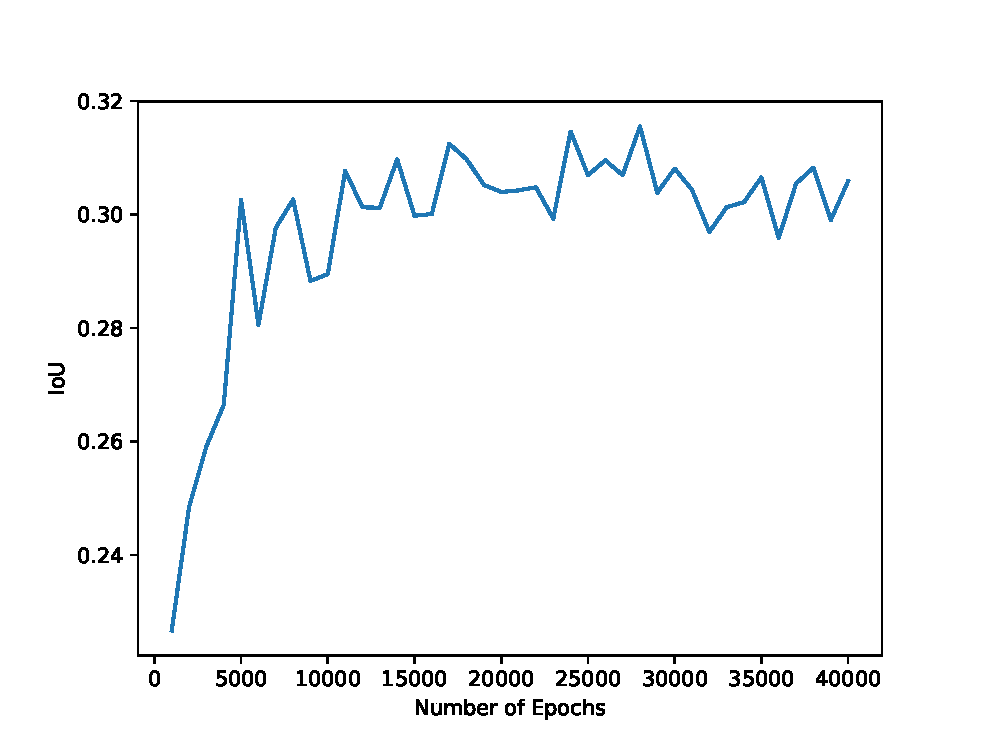
\includegraphics[scale=0.5]{results/conf1.eps}
	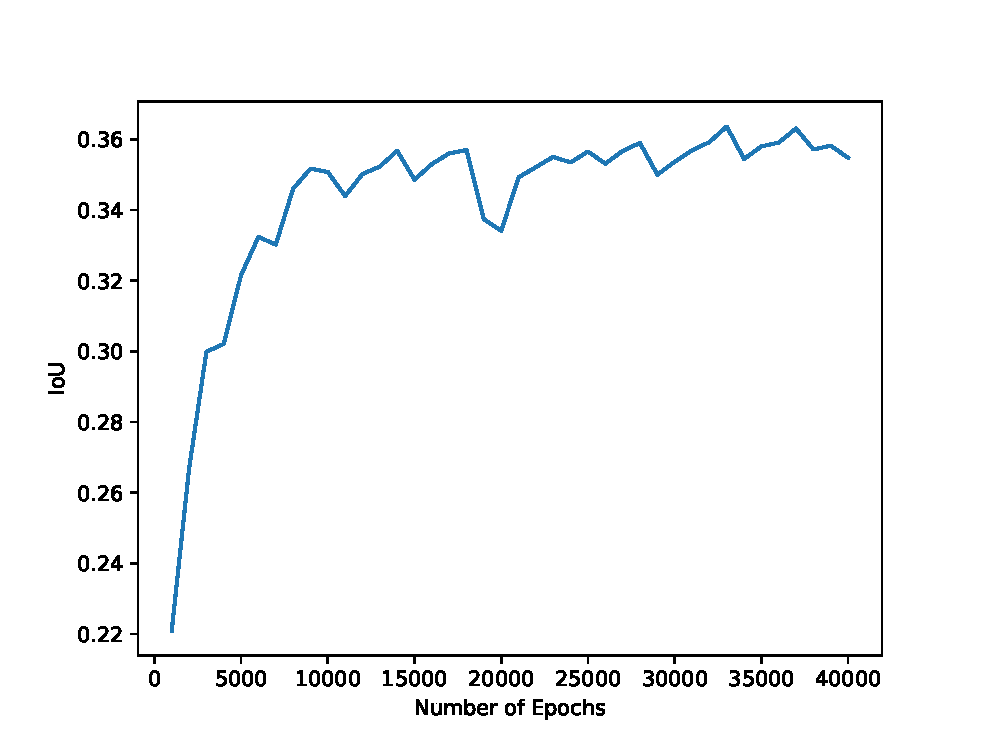
\includegraphics[scale=0.5]{results/conf4.eps}
	\caption{IoU over epochs/iterations for Configuration 1 (left) and Configuration 4 (right)}
\end{figure}
We see that both experiments converge rather quickly and that the configuration with the skip connections outperforms the baseline without skip connections. The best IoU values where 0.315 (Configuration 1) and 0.364 (Configuration 4).



\end{document}


